\subsection{一致结构的定义}

定义 1 集合 X 上的一致结构（或一致）是这样的结构：它由 X × X 的一个子集族 U 给出，该子集族满足第一章 § 6 第 1 目的公理（F\_I）与（F\_II），并且还满足下列公理：

\((\mathbf{U}_{\mathbf{I}})\) 属于 \(\mathfrak{U}\) 的每个集合都含对角线 \(\Delta\)。

\((\mathbf{U}_{\mathbf{II}})\) 若 \(\mathbf{V}\in \mathfrak{U}\)，则 \(\overline{\mathbf{V}}^1\in \mathfrak{U}\)。

\((\mathbf{U}_{\mathbf{III}})\) 对每个 \(\mathbf{V} \in \mathfrak{U}\)，存在 \(\mathbf{W} \in \mathfrak{U}\) 使 \(\mathbf{W} \circ \mathbf{W} \subset \mathbf{V}\)。

\pandocbounded{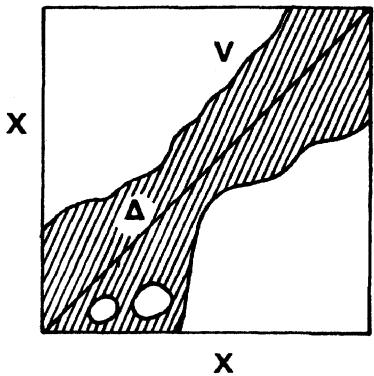
\includegraphics[keepaspectratio]{images/part001_6ce88dc6.jpg}}\\
图 2.

\(\mathfrak{U}\) 中的诸集合称为在 \(\mathbf{X}\) 上由 \(\mathfrak{U}\) 所定义的一致结构的一致邻域。赋有一致结构的集合称为一致空间。

若 V 是集合 X 上某个一致结构的一致邻域，我们可以把关系 \((x, x') \in V\) 表述为“x 与 \(x'\) 是 V-邻近的”。

注。1）为使语言更富表现力，我们可以在某些陈述中使用“x 与 y 足够接近”“x 与 y 要多接近就有多接近”这类说法。例如，我们将说，一个关系

R \(\{x,y\}\) 只要 x 与 y 足够接近便为真，如果存在一致邻域 V，使关系 \((x,y)\in V\) 蕴含 R \(\{x,y\}\)。

\begin{enumerate}
\def\labelenumi{\arabic{enumi})}
\setcounter{enumi}{1}
\tightlist
\item
  公理（U \(_{II}\)）与（U \(_{III}\)）的合取（在一致结构的其余公理之下）等价于下述公理：
\end{enumerate}

\((\mathbf{U}_a)\) 对每个 \(\mathbf{V} \in \mathfrak{U}\)，存在 \(\mathbf{W} \in \mathfrak{U}\) 使 \(\mathbf{W} \circ \overline{\mathbf{W}} \subset \mathbf{V}\) (*)。

显然 \((\mathbf{U}_{\mathrm{II}})\) 与 \((\mathbf{U}_{\mathrm{III}})\) 蕴含 \((\mathbf{U}_a)\)。反之，若 \((\mathbf{U}_a)\) 成立，我们有 \(\overline{\mathbf{W}} = \Delta \circ \overline{\mathbf{W}} \subset \mathbf{V}\)（由 \((\mathbf{U}_I)\)）；于是 \(\mathbf{W} \subset \overline{\mathbf{V}}\)，从而{[}由 \((\mathbf{F}_I)] \overline{\mathbf{V}} \in \mathfrak{U}\)。令 \(\mathbf{W}' = \mathbf{W} \cap \overline{\mathbf{W}}\)；则 \(\mathbf{W}' \in \mathfrak{U}\)（由刚才所证及公理 \((\mathbf{F}_{\mathrm{II}})\)），并且 \(\mathbf{W}' \circ \mathbf{W}' \subset \mathbf{W} \circ \overline{\mathbf{W}} \subset \mathbf{V}\)。

本章中我们始终用 \(\mathbf{V}\) 代替 \(\mathbf{V} \circ \mathbf{V}\)，一般地写 \(\mathbf{V} = \mathbf{V} \circ \mathbf{V} = \mathbf{V} \circ \mathbf{V}\)，其中 \(n > 1\) 为整数，\(\mathbf{V}\) 为 \(\mathbf{X} \times \mathbf{X}\) 的子集。

\begin{enumerate}
\def\labelenumi{\arabic{enumi})}
\setcounter{enumi}{2}
\tightlist
\item
  若 X 非空，则公理 \((U_{I})\) 蕴含 U 中没有一个集合是空集，从而 U 是 \(X \times X\) 上的一个滤子。空集上只有一个一致结构，即 \(U = \{\varnothing\}\)。
\end{enumerate}

定义 2 一致结构的一致邻域基本系是指由一致邻域组成的任一这样的族 B：每个一致邻域都含有属于 B 的一个集合。

公理 \((\mathbf{U}_{\mathbf{III}})\) 表明，若 n 为任一整数 \textgreater0 且 V 取遍某个一致邻域基本系，则诸集合 \(V^{n}\) 仍构成一个一致邻域基本系。

满足 \(V = \overline{V}^{1}\) 的一致邻域 V 称为对称的。若 V 是任一一致邻域，则 \(V \cap \overline{V}^{1}\) 与 \(V \cup \overline{V}^{1}\) 都是对称一致邻域，并且公理 \((F_{\mathrm{II}})\) 与 \((U_{\mathrm{II}})\) 表明诸对称一致邻域构成一个一致邻域基本系。

子集族 \(\mathfrak{B}\)——它由 \(\mathbf{X} \times \mathbf{X}\) 的子集组成——是 \(\mathbf{X}\) 上某个一致结构的一致邻域基本系，当且仅当 \(\mathfrak{B}\) 满足第一章 § 6 第 3 目的公理（ \(B_{\mathbf{I}}\)），并且还满足下列公理：

\((\mathbf{U}_{\mathbf{I}}^{\prime})\) \(\mathfrak{B}\) 中的每个集合都含对角线 \(\Delta\)。

\((\mathbf{U}_{\mathbf{II}}^{\prime})\) 对每个 \(\mathbf{V} \in \mathfrak{B}\)，存在 \(\mathbf{V}' \in \mathfrak{B}\) 使 \(\mathbf{V}' \subset \overline{\mathbf{V}}^1\)。

\((\mathbf{U}_{\mathbf{III}}^{\prime})\) 对每个 \(\mathbf{V} \in \mathfrak{B}\)，存在 \(\mathbf{W} \in \mathfrak{B}\) 使 \(\tilde{\mathbf{W}} \subset \mathbf{V}\)。

若 X 非空，则 X 上一致结构的一致邻域基本系是由该结构的诸一致邻域组成的滤子的一个基（第一章 § 6 第 3 目命题 3）。

(*) 我们回顾（《集合论》，R，§ 3，第 4 与第 10 目）：若 V 与 W 是 \(\mathbf{X} \times \mathbf{X}\) 的两个子集，则由对 \((x, y) \in \mathbf{X} \times \mathbf{X}\)（它们满足：\((x, z) \in \mathbf{W}\) 且 \((z, y) \in \mathbf{V}\) 对某个 \(z \in \mathbf{X}\) 成立）组成的集合记作 V o W 或 VW，而由对 \((x, y) \in \mathbf{X} \times \mathbf{X}\) 中满足 \((y, x) \in \mathbf{V}\) 者组成的集合记作 \(\overline{\mathbf{V}}\)。

一致结构的例子。* 1）在实数集 R 上可以如下定义一个称为加法一致结构的一致结构：对每个 \(\alpha > 0\)，令 \(V_{\alpha}\) 为 \(R \times R\) 中由对 \((x, y)\)（满足 \(|x - y| < \alpha\)）全体组成的子集；当 \(\alpha\) 取遍一切实数 \(> 0\) 时，诸 \(V_{\alpha}\) 构成 R 上加法一致结构的一个一致邻域基本系。类似地，在有理数集 Q 上可以定义一个一致结构（也称加法一致结构）；我们将在第三章与第四章中研究这些结构以及群上类似的一致结构。* 2）设 X 是一个集合，R 是 X 上的一个等价关系；令 C 为

R 在 \(\mathbf{X} \times \mathbf{X}\) 中的图像。于是 \(\Delta \subset \mathbf{C}\) 且 \(\tilde{\mathbf{C}} = \tilde{\mathbf{C}} = \mathbf{C}\)（《集合论》，R，§ 5，第 1 目）；因此由单独一个集合 C 组成的 \(\mathbf{X} \times \mathbf{X}\) 的子集族是 X 上某个一致结构的一致邻域基本系。特别地，若取 R 为相等关系，则 \(\mathbf{C} = \Delta\)，而相应一致结构的诸一致邻域是 \(\mathbf{X} \times \mathbf{X}\) 中含 \(\Delta\) 的一切子集；这个一致结构称为 X 上的离散一致结构，赋有这个一致结构的集合 X 称为离散一致空间。

\begin{enumerate}
\def\labelenumi{\arabic{enumi})}
\setcounter{enumi}{2}
\tightlist
\item
  在有理整数集 \(\mathbf{Z}\) 上可以如下定义一个在数论中重要的一致结构：给定一个素数 \(p\)，令 \(\mathbf{W}_n\) 为由对 \((x,y)\in \mathbf{Z}\times \mathbf{Z}\) 中满足 \(x\equiv y\)（mod \(p^n\)）者全体组成的集，这里 \(n > 0\) 为任意整数。容易验证，诸集合 \(\mathbf{W}_n\)（对固定的 \(p\)）构成 \(\mathbf{Z}\) 上某个一致结构的一致邻域基本系，该一致结构称为 \(p\) 进一致结构（参看第三章 § 6 习题 23 及以后，以及第九章 § 3 第 2 目）。
\end{enumerate}

按照一般的定义（《集合论》，R，§ 8，第 5 目），若 X 与 X' 是两个各赋有一致结构的集合，其一致邻域族分别为 U 与 U'，则 X 到 X' 上的双射 f 是 X 的一致结构到 X' 的一致结构上的同构，如果 g(U) = U'，其中 g = f × f。

例如，若 X 与 \(X'\) 是两个等势的集合，则 X 到 \(X'\) 上的每个双射都是 X 的离散一致结构到 \(X'\) 的离散一致结构上的同构。

